\begin{tikzpicture}

  % ── Estilos baseados no manual do TikZ ────────────────────────
  \tikzset{
    apoio/.style = {draw, thick},
    carga/.style = {draw=red, -Latex, thin}, % Requer a biblioteca arrows.meta
    diagrama/.style = {fill=gray!15, draw=blue!0, thick}
  }

  % =========================================================
  % 2. DIAGRAMA DE MOMENTO FLETOR (DMF)
  % =========================================================
  
  % Deslocamos o diagrama para baixo para não sobrepor a viga
  \begin{scope}[yshift=-3.5cm]
    
    % Eixo neutro do diagrama (linha horizontal)
    \draw[thick] (0,0) -- (14.4,0) node[right, font=\small\bfseries] {DMF};
    
    % Linhas guias descendo dos apoios e do final do balanço
    %\draw[dashed, gray] (0, 3.5) -- (0, 0);
    %\draw[dashed, gray] (4, 3.5) -- (4, -2.5);
    %\draw[dashed, gray] (6, 3.5) -- (6, 0);

    % Curvas do Momento Fletor
    % Nota: Para desenhar o momento positivo para BAIXO, multiplicamos as equações por -1.
    % Equação vão A-B (x de 0 a 4): M(x) = 1.5x - 0.5x^2  --> y = - (1.5x - 0.5x^2)
    % Equação balanço (x de 4 a 6): M(x) = 6x - 0.5x^2 - 18 --> y = - (6x - 0.5x^2 - 18)
    \filldraw[diagrama] 
      (0,0) 
      -- plot[domain=0:10, samples=50] (\x, {-3*\x + 1*\x*\x}) 
      -- plot[domain=10:14.4, samples=50] (\x, {-3*\x + 1*\x*\x + 36}) 
      -- (14.4,0) -- cycle;

    % Rótulos dos valores notáveis de Momento
    
    % 1. Momento Máximo Positivo no vão (Ocorre em x=1.5, onde V=0)
    %\draw[dashed, gray] (1.5,0) -- (1.5, -1.125);
    \node[below, text=blue!80!black] at (5.5, -1.125) {$91$};
    
    % 2. Momento Máximo Negativo (No apoio B, x=4)
    \node[above, text=blue!80!black] at (12.5, 2) {$108,4$};
    %\filldraw[blue!80!black] (12.2, 2) circle (1.5pt);

    % 3. Zeros nas extremidades
    %\node[left, blue!80!black] at (0,0) {$0$};
    %\node[right, blue!80!black] at (6,0) {$0$};
    
    % Símbolos de + e - dentro do diagrama
    %\node[blue!80!black] at (1.5, -0.5) {\large $+$};
    %\node[blue!80!black] at (4.5, 0.5) {\large $-$};

  \end{scope}

\end{tikzpicture}

\begin{comment}
    Perfil caixão
    Duplo perfil I

    Exercícios propostos

    FLEXÃO      CORTE
    6.2.4       7.2.1
    6.2.5       7.3.1
    6.3.1       7.3.3
    6.3.4       7.

    Três questões da acima, e são três questões na prova
\end{comment}